\section{O Programa}

Além das bibliotecas padrão de Python, foram utilizados os pacotes SciPy \autocite{ref:scipy} e OpenCV \autocite{ref:opencv}.

\subsection{Código Fonte}

    O programa foi desenvolvido em Python 3.8, mas deveria funcionar com as versões 3.6 e 3.7 também. Além disso, o código fonte foi separado nos seguintes arquivos:

    \begin{description}
        \item[main.py] É o corpo do programa, resposável por processar os comandos e opções da linha de comando.

        \item[lib.py] Funções de tranformação da imagem, como ajuste de brilho e acesso do plano de bits.

        \item[filtro.py] Definição das máscaras de convoluções (\textit{kernels}).

        \item[inout.py] Funções que tratam da entrada e saída do programa, como leitura e escrita de arquivos de imagem e também da apresentação da imagem em uma janela gráfica.

        \item[tipos.py] Definição dos tipos para checagem estática com \texttt{mypy} \autocite{ref:mypy}.
    \end{description}

    Todas as figuras base utilizadas neste relatório podem ser encontradas na pasta \texttt{imagens} do código fonte, como descrito nos rótulos da \cref{fig:base}. Além disso, foi disponibilizado também um \textit{script} em \texttt{bash}, \texttt{run.sh}, que realiza todos os processamentos requeridos em cada uma das imagens na pasta.

\subsection{Execução} \label{sec:execucao}

    A execução deve ser feita através do interpretador de Python 3.6+. A única entrada obrigatória é o caminho para a imagem PNG que será processada. As entradas seguintes devem ser os \textit{kernels} de convolução, no formato \texttt{h1} até \texttt{h11}. Ao final da execução, a imagem resultante será exibida na tela. Por exemplo, o comando abaixo apresenta a \cref{fig:execucao} em uma nova janela gráfica.

    \begin{minted}{text}
        $ python3 main.py imagens/baboon.png h1 h2
    \end{minted}

    \begin{figure}[H]
        \centering
        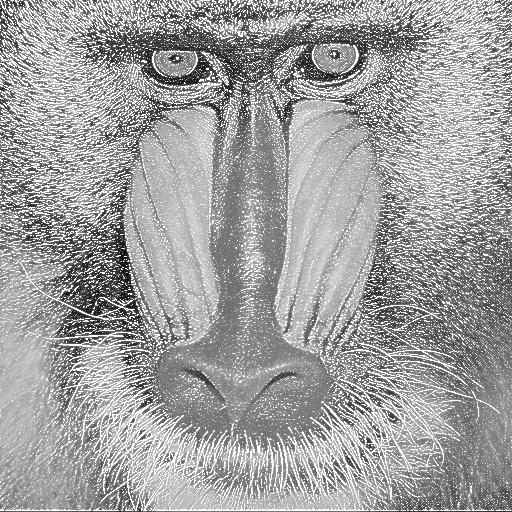
\includegraphics[width=6cm]{resultados/execucao.png}

        \caption{Aplicação de alguns processamentos na \texttt{baboon.png}.}
        \label{fig:execucao}
    \end{figure}

    Além das entradas posicionais, existem algums argumentos opicionais, que podem ser vistos com \mintinline{bash}{$ python3 main.py --help}. A mais importante das opções é \mintinline{text}{--output}, ou \mintinline{text}{-o}, que salva o resultado em um arquivo PNG em vez de exibir na tela. Se é desejável tanto a exibição da imagem quanto o salvamento no arquivo, o argumento \mintinline{text}{--force-show} ou \mintinline{text}{-f} pode ser usado. As outras opções são referentes ao \textit{kernel} de convolução e serão descritas na \cref{sec:resultado}.
